% This abstract was made as part of the Academic Argumentation Skills in Writing and Debate MOS module.
\documentclass[a4paper,12pt]{article}
\usepackage{fontspec}
\usepackage[usenames,dvipsnames]{color}
\usepackage{soul} % Highlighting in colour
\usepackage{endnotes} % Multiple footnotes
\usepackage{hyperref} % Doesn't seem to work...

% This should be 1.241 for one-and-half spacing, but it causes text to spill over to another page, so use a less silly amount of spacing
\linespread{1.05}
% For proper endnotes
\def\enoteheading{\noindent\rule{.5\textwidth}{0.4pt}}

\title{Comparison of machine learning algorithms for fuzzy land cover classification}
\author{Dainius Masiliūnas}

\begin{document}

\maketitle

\begin{center}
 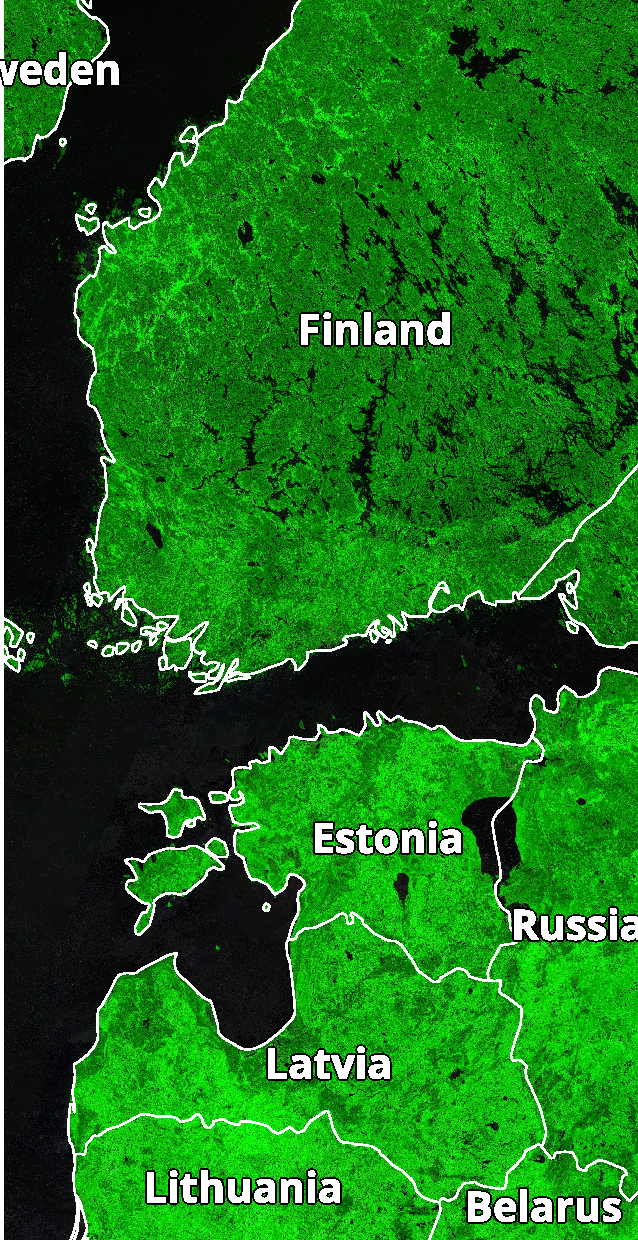
\includegraphics[width=0.5\textwidth]{thesis-figures/aoi-blank}
\end{center}

\pagebreak

% When introducing an abbreviation, capitalise and underline the first letter.
\begin{abstract}
The current standard of land cover classification is to assign each pixel to one land cover class, which at coarse resolution causes loss of information about mixed land cover. Fuzzy land cover classification, which assigns fractions of each land cover class to each pixel, can deal with mixed pixels. However, so far its application has been limited to city-scale areas, four or fewer classes, and up to two algorithm comparisons. In this paper, the classification accuracy and processing speed were compared for three fuzzy classification machine learning algorithms: random forest regression, fuzzy \textit{c}-means and neural networks. The algorithms were used to classify the whole boreal-temperate forest gradient zone between Finland and Lithuania into nine land cover classes. Results showed that all of the tested algorithms are able to achieve similarly high classification accuracy. Random forest regression accuracy was the highest, but its processing speed was the lowest. The results are a milestone for creating a global fuzzy land cover classification product incorporating user-specific requirements.
\end{abstract}

\pagebreak

\let\footnotemark=\endnotemark
\let\footnotetext=\endnotetext
\renewcommand{\abstractname}{Extended abstract}
\newcommand{\claim}[1]{\sethlcolor{yellow}\hl{#1}\footnotemark[1]}
\footnotetext[1]{Toulmin's argumentation model: Claim.}
\newcommand{\data}[1]{\sethlcolor{SkyBlue}\hl{#1}\footnotemark[2]}
\footnotetext[2]{Toulmin's argumentation model: Data.}
\newcommand{\warrant}[1]{\sethlcolor{green}\hl{#1}\footnotemark[3]}
\footnotetext[3]{Toulmin's argumentation model: Warrant.}
\newcommand{\backing}[1]{\sethlcolor{Apricot}\hl{#1}\footnotemark[4]}
\footnotetext[4]{Toulmin's argumentation model: Backing.}
\newcommand{\qualifier}[1]{\sethlcolor{Orchid}\hl{#1}\footnotemark[5]}
\footnotetext[5]{Toulmin's argumentation model: Qualifier.}
\newcommand{\acknowledgement}[1]{\sethlcolor{LimeGreen}\hl{#1}\footnotemark[6]}
\footnotetext[6]{Toulmin's argumentation model: Acknowledgement.}
\newcommand{\rebuttal}[1]{\sethlcolor{Lavender}\hl{#1}\footnotemark[7]}
\footnotetext[7]{Toulmin's argumentation model: Rebuttal.}

\begin{abstract}
\data{The current standard way of classifying land cover is to assign each pixel to one land cover class (hard classification).} \backing{Since this is usually done on 300×300 m pixels, most of which represent mixed land cover,} \claim{hard classification distorts the actual area covered by a particular class.} \claim{Fuzzy land cover classification should be used instead of hard classification,} \data{because it assigns fractions of each land cover class to each pixel and thus is able to accurately express mixed pixels.} \warrant{Accurate representation of mixed land cover is important} \backing{for climate modelling, land monitoring and other fields.} However, so far fuzzy classification has been limited to city-scale areas, four or fewer classes, and up to two algorithm comparisons. In this paper, the classification accuracy and processing speed were compared for three fuzzy classification machine learning algorithms: random forest regression, fuzzy \textit{c}-means, neural networks. While there is a variety of algorithms available, \claim{these three were chosen as fitting the study best because} \data{they are radically different from one another.} \warrant{Testing a variety of methods is useful from a statistics viewpoint} \backing{as it allows inferring results about related algorithms.} The algorithms were used to classify the whole boreal-temperate forest gradient zone between Finland and Lithuania into nine land cover classes. \claim{This is a representative area for land cover classification} \data{because it covers an area of 10×10°} \warrant{which is large enough} \backing{to include all nine major land cover classes.} Results showed that all of the tested algorithms are able to achieve similarly high classification accuracy. Random forest regression accuracy was the highest (mean absolute error: 11.7\%), but its processing speed was the lowest. \claim{The results are a milestone for creating a global fuzzy land cover classification product incorporating user-specific requirements,} \data{since the algorithms can be used to perform fuzzy land cover classification at a global scale.} \acknowledgement{While the fuzzy classification method requires extra data from which to discern the subpixel land cover fractions,} \rebuttal{this is usually covered by time series data and globally available data, such as elevation.}
\end{abstract}

\theendnotes

\pagebreak

% Mention why it's not pre-science.
% Incorporate information on how it's important for other fields (which).
\section*{Memo}
\claim{The paper is classified as science rather than pseudoscience,} \data{since it tests the hypothesis of whether and which fuzzy classification algorithms can be applied to a large number of classes and at a large extent.} \warrant{Popper considers falsifiability as the main criterion for discerning science from pseudoscience,} \backing{and in this case algorithm applicability could be disproved by a low prediction accuracy statistic compared to the others,} \backing{whereas the fuzzy classification paradigm as a whole could be disproved as unnecessary by a comparably high hard classification accuracy statistic.} \claim{The paper should} \qualifier{probably} \claim{be classified as normal rather than revolutionary science,} \data{since the method, while innovative, had already been successfully applied on smaller datasets in other papers.} \warrant{Only high-impact works that introduce a change in the prevalent paradigm are revolutionary science,} \backing{according to Kuhn,} \acknowledgement{and while the fuzzy classification paradigm might displace hard classification in the future,} \rebuttal{this paper is not aimed for and thus is not likely to be the driving force for the change by itself.} \claim{It is also not pre-science,} \data{since methods proposed by previous studies are applied at a much larger scale in this paper.} \claim{It is standard science,} \data{since the methodology is strict and well-defined.} \warrant{The alternative, random science, does not follow a stringent, rational method,} \backing{according to Feyerabend.} \claim{The paper is post-modern science,} \data{since the focus is on creating a new method for monitoring land cover by taking into account and expressing more of the natural world complexity.} \data{In addition, the target audience is the scientific community with per-user requirements, which allows the land cover product to be user-adjustable and thus have a broader interdisciplinary reach.} \backing{Taking the complexity into account, rather than attempting to minimise and ignore it,} \backing{and interdisciplinary, user-oriented approach, rather than disciplinary, knowledge-oriented approach,} \warrant{are all traits associated with post-modern rather than traditional science.}

\theendnotes

\end{document}
